\documentclass[a4paper]{article}

\usepackage[margin=1in]{geometry}
\usepackage{graphicx}
\usepackage{fancyhdr}
\usepackage{hyperref}

\newcommand{\theDate}{July  29th, 2017} %Change this every meeting
\setlength{\headheight}{13.6pt}
\pagestyle{fancy}
\fancyhf{}
\fancyfoot[L]{ECE 4600 Project Proposal}
\fancyfoot[R]{\theDate{}}
\fancyfoot[C]{\thepage}

\begin{document}
	\begin{center}
		\huge Autonomous Robot Cluster
	\end{center}
	\textbf{Team} Farhan Rahman, Wyatt Thomson, Huy Bui, James Jo, Aleksa Svitlica \\

	\section*{Description}
		\par 
		The objective of our proposed project is to create a smart network capable of routing robots optimally. The robots are intended to represent vehicles and they themselves can be as simple or complicated as desired. \par
		The smart network will employ machine learning to improve routing and be able to adapt to different configurations roads. When a robot approaches the intersection it would communicate to the network and receive instructions about whether it should continue, slow down, stop or any other reasonable instruction. The network would make these decisions based on information about other robots approaching the intersections, robot speeds and their intended paths. To keep track of all the robots as they move around we are looking in to a machine vision solution; potentially having a single camera watching over the robots and relaying information to the computer which can then determine position and velocity of the robots. \par
		For communication between the network and individual robots we are currently considering ZigBee and MiWi protocls.The ZigBee protocol is most commonely seen in remotes and smart home electronics. MiWi is a protocol created and distributed by Microchip and is advertised as a smaller footprint alternative to ZigBee. Communication between the base station and our computer will likely be through a USB interace.\par
		The robots which we are using to simulate vehicles will be relatively simple. We have began narrowing down the specifications and already have a microcontroller, motors and transceiver picked out pending final evaluations. Routing and driving of the robots is still very much under discussion. We could hard program how to driver straight, do simple turns and anything else basic or we could apply machine learning here too. The benefit of using machine learning here is that we could theoretically use any sort of road system and would allow for much more complicated tests later during the smart network phase. \\  
		 
	\section*{Roadmap}
	Note: Roadmap is subject to change based on finalization of project requirements and scope.
	\begin{itemize}
		\item \textbf{August:}
			\begin{itemize}
				\item \textbf{Finalize Project Scope} As it stands our project has the potential to have very many tasks, the first one is to decide what we our exact requirements and goals are. This is when we decide on large requirements like whether to use machine learning for the robot driving or whether we are using ZigBee or MiWi.
			\end{itemize}
		\item \textbf{September:}
			\begin{itemize}
				\item \textbf{Research ZigBee/MiWi}
				\item \textbf{Research and setup test neural network} This would be a neural net solving something much simpler than our project. Learn the foundation and apply it to something basic.
				\item \textbf{Finalize hardware choices} We want to decide on the MCU, motors and transceiver for the robots; as well as the hardware for the base station (smart network).
			\end{itemize}
		\item \textbf{October:}
			\begin{itemize}
				\item \textbf{Prototype robot and base station} Assemble at least one robot and the base station so coding and testing on them can begin.
				\item \textbf{Camera tracking} Begin researching and potentially testing tracking of the robots with a camera.
				\item \textbf{Driving Simulation} Begin work on a software simulation of the robots driving. Be able to hard code directions or potentially start applying machine learning.
			\end{itemize}
		\item \textbf{November:}
			\begin{itemize}
				\item \textbf{Camera tracking continued} Begin testing of camera tracking and relaying information to the base station
				\item \textbf{Network} Setup communication between base station and a robot. Setup communication between base station and computer.
				\item \textbf{Simulations} Continue work on driving simulation and begin work on smart network intersection routing simulation
			\end{itemize}
		\item \textbf{December:}
			\begin{itemize}
				\item \textbf{Full system} Begin testing system of driving robot with camera tracking and some sort of communication with base station.
				\item \textbf{Neural Net Testing} If simulations are successful begin transition from software test to real world test.
				\item \textbf{Evaluation} Determine what has been completed, what needs to be completed and what else would we like to do if we have time. At this point decide on Winter semester roadmap.
			\end{itemize}
		\item \textbf{January:}
			\begin{itemize}
				\item Pending December evaluation.
			\end{itemize}
		\item \textbf{February:}
			\begin{itemize}
				\item \textbf{Work on presentation/report}
			\end{itemize}
		\item \textbf{March:}
			\begin{itemize}
				\item 
			\end{itemize}
	\end{itemize}
	\section*{Citations}
	Here is a list of some preliminary research which we believe shows our project is reasonable:\\
	
	\textbf{Stanley and Miikkulainen, 2002] Stanley, K., and Miikkulainen, R., “Evolving Neural Networks through Augmenting Topologies”. Evolutionary Computation Volume 10, Number 2, 2002.}\\
	”This paper is about a method of neural network implementation that outperforms traditional neural nets."\\ 
	\href{http://nn.cs.utexas.edu/downloads/papers/stanley.ec02.pdf}{Link}\\
		
	\textbf{[Aerospace Controls Lab, 2015], Aerospace Controls Lab., “Autonomous Drifting using Machine Learning.” 2015.}\\
	“This video shows both the ability to train a small RC car to do a task much more complex than what we intend. Additionally they also demonstrate tracking of the RC cars with a camera; this is something we intend to emulate." \\
	\href{https://www.youtube.com/watch?v=opsmd5yuBF0}{Link}\\
		
	\textbf{[Hadik, 2013] Hadik, A. “MATLAB Neural Network Autonomous Car”, 2015.}\\
	"Another autonomous RC car This video shows students using machine learning to train a car to predict a path based on image data. We might potentially do something similar if we decide to apply machine learning to the robots."\\
	\href{https://www.youtube.com/watch?v=mW6Y\_tiiNYM}{Link}\\
		
	\textbf{[Wan et al., 2009] Wan, J., Wang, Y., Qin, Q., and Li, Y. “Multi-Robots’ Communication System Based On ZigBee Network”. In The Ninth International Conference on Electronic Measurement \& Instruments, 2009.}\\
	"Publication in ICEMI 2009. Similar to our project of robot network cluster. Showcases Network structure, hardware implementation and communications function."\\ \href{http://ieeexplore.ieee.org.uml.idm.oclc.org/document/5274350/}{Link}\\
		
	\textbf{[Surmann et al., 2014] Surmann, H., Worst, R., Zimmermann, E., Wilkes, S., Liebelt, T., and Eulering, C. “Simple Mobile Robots and Self-Adaptive Wireless Networks”. In 41st International Symposium on Robotics, 2014.}\\
	“Publication in International Symposium on Robotics Gives a case study for Robot networks in disaster areas.\\ 
	\href{http://ieeexplore.ieee.org.uml.idm.oclc.org/document/6840176/}{Link}\\
	
	\textbf{Kay, Russell. (2006). ZigBee.(QUICK STUDY). Computerworld, 40(20), 46-46.}\\
	"Encryption based on the AES-128 standard certified by National Institution of Standards and
	Technology."\\
	
	\textbf{Tachet R, Santi P, Sobolevsky S, Reyes-Castro LI, Frazzoli E, Helbing D, et al. (2016) Revisiting Street Intersections Using Slot-Based Systems. PLoS ONE 11(3): e0149607.}\\
	"Apply Street Intersections using slot-based systems technique (research by MIT)."\\
	\href{https://doi.org/10.1371/journal.pone.0149607}{Link}\\
	
	\section*{Bill of Material}
	Note: This is a preliminary estimation of what we would be expecting to spend. Subject to change or increase. All Prices in CAD. \\
	Per robot unit: \\
	
	\textbf{PIC18F45K40-I/P-ND – \$3.11} \\
	Description: 40-Pin 8-bit MCU unit from MicroChip. Reason for using this MCU is that there is a familiar IDE for use with the line of product, and there is also a IEEE 802.15.4 compatible Tranciever that we would want to use in this project.
	URL: https://www.digikey.ca/short/3vhwbw \\
	
	\textbf{MRF24J40MAT-I/RMCT-ND Unit – \$14.70} \\
	Description: MicroChip brand RF Tranciever Module, for this project we are hoping to use IEEE Standard 802.15.4 radios to creat a network of functional robots, more specificaly we are hoping to use a popular protocol known as ZigBee to achive this. \\
	
	This RF module is compatable with ZigBee and we hope to use this to connect to the SPI interface of our MCU unit. The RF module will send instructions to the MCU to make it carry out tasks. \\
	
	There are many RF modules to chose from, so we may experiment and research others while working on the project.
	URL: https://www.digikey.ca/short/3vhwbf \\
	
	
	\textbf{Motor x2 - \$0.59} \\
	Description: Simple DC Motor, we would use an H-Bridge circuit to properly drive the control of the motors, would use simple controls to control direction of robot. \\ \\
	
	\textbf{L293D H-Bridge Circuit - \$0.45} \\
	Description: H-Bridge Circuit IC. Since we are trying to build a simple car, we would control the two motors and their direction using a simple H-Bridge IC. It would be directly connected to the MCU's GPIO. \\
	\begin{figure}[h]
		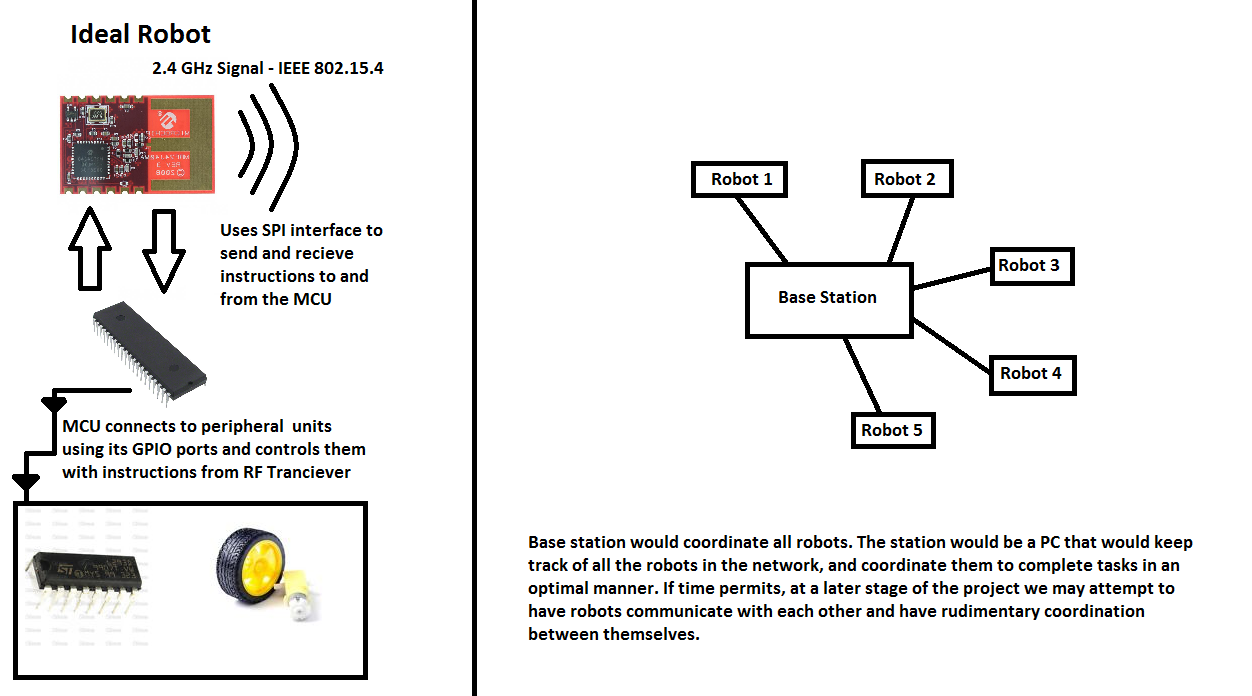
\includegraphics[scale=0.5]{../diag.png}
		\caption{Simple diagram of our planned system}
	\end{figure}
\end{document}
